\chapter{Algebra Relazionale}

\section{Linguaggi per basi di dati}
\begin{center}
	Operazioni sullo schema $\rightarrow$ \textbf{DDL}:\ \textbf{Data Definition Language}
\end{center}

\noindent Operazioni di creazione, cancellazione e modifica di schemi di tabelle, creazione viste, creazione indici\dots

\begin{center}
	Operazioni sui dati $\rightarrow$ \textbf{DML}:\ \textbf{Data Manipulation Language}
\end{center}

\begin{itemize}
	\item Data Query language:\ query o interrogazione della base di dati
	\item Aggiornamento dati:\ inserimento, cancellazione e modifica di dati
\end{itemize}

\subsection{Linguaggi Relazionali}

\textit{\textbf{Algebra} relazionale}:\ insieme di operatori su relazioni che danno come risultato relazioni.\
Non si usa come linguaggio di interrogazione dei DBMS ma come rappresentazione interna delle interrogazioni.

\textit{\textbf{Calcolo} relazionale}:\ linguaggio dichiarativo di tipo logico dal quale è stato derivato l'SQL.

\noindent Operatori dell'algebra relazionale
\begin{itemize}
	\item unione, intersezione, differenza;
	\item ridenominazione;
	\item selezione;
	\item proiezione;
	\item join (join naturale, prodotto cartesiano, theta-join).
\end{itemize}
Operatori insiemistici
\begin{itemize}
	\item le relazioni sono insiemi
	\item i risultati devono essere relazioni
\end{itemize}
è possibile applicare \textbf{unione}, \textbf{intersezione}, \textbf{differenza} solo a relazioni definite sugli stessi attributi, cioè possono operare solo su tuple uniformi.

\begin{figure}[H]
	\centering
	\caption*{Unione:\ $\cup$}
	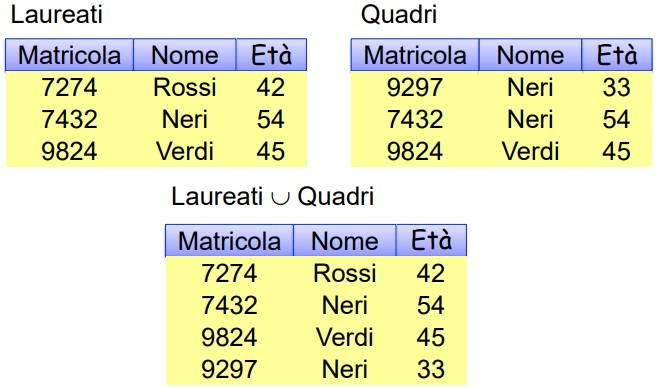
\includegraphics[width=0.5\textwidth]{immagini/AR_unione.jpg}

	\caption*{Intersezione:\ $\cap$}
	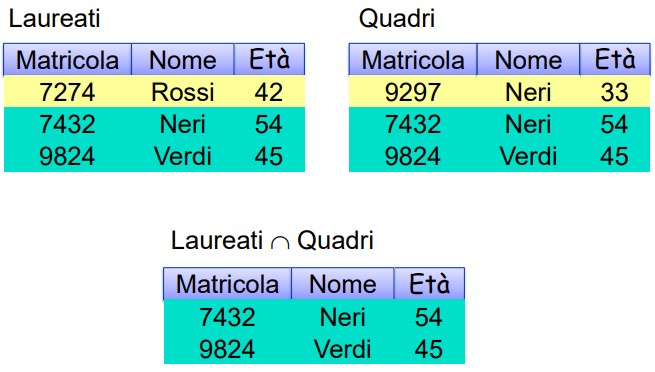
\includegraphics[width=0.5\textwidth]{immagini/AR_intersezione.jpg}

	\caption*{Algebra Relazionale:\ Differenza}
	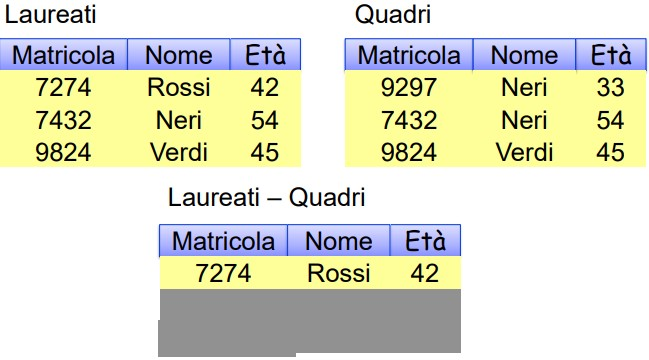
\includegraphics[width=0.5\textwidth]{immagini/AR_differenza.jpg}
\end{figure}

\subsubsection{Ridenominazione}

Operatore monadico (con un argomento), ``modifica lo schema'' lasciando inalterata l'istanza dell'operando.

È indicato con la lettera $\rho$

\begin{figure}[H]
	\centering
	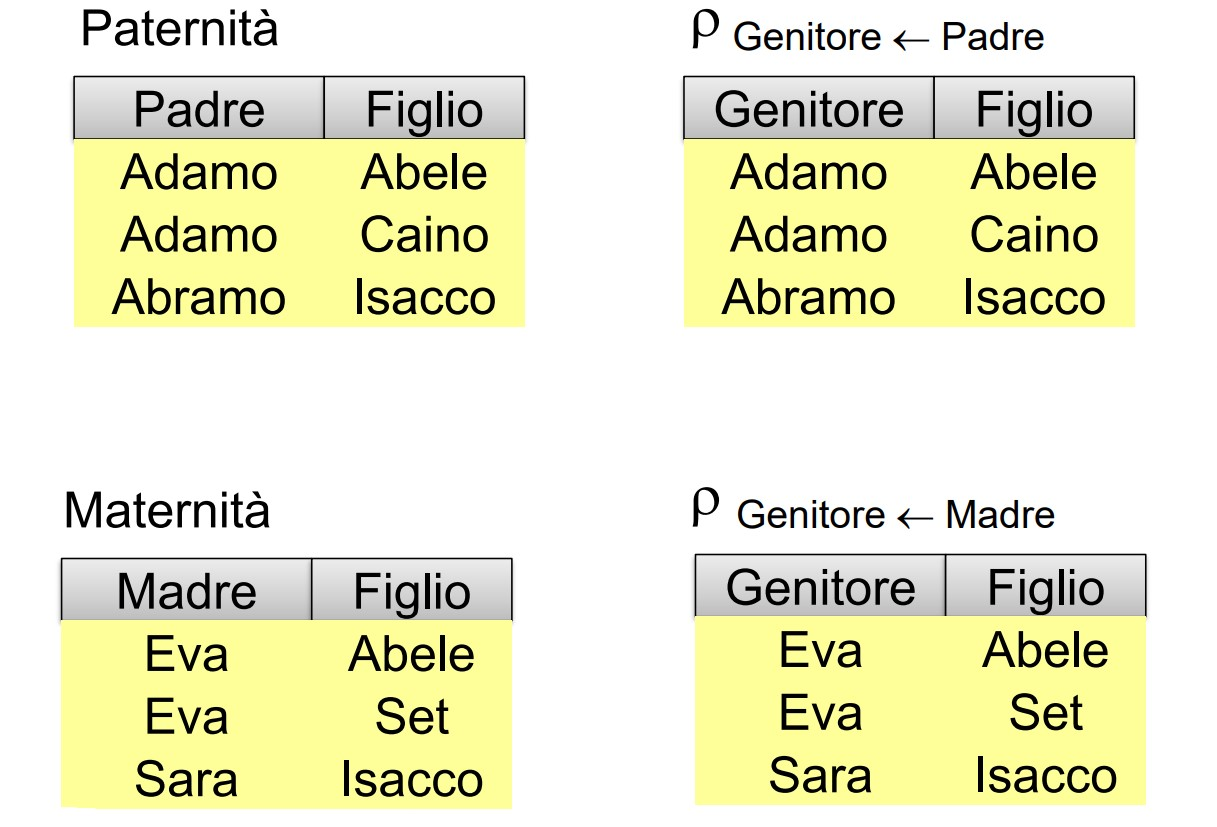
\includegraphics[width=0.5\textwidth]{immagini/AR_ridenominazione.jpg}
\end{figure}

\subsubsection{Proiezione}

Operatore monadico, produce un risultato che ha parte degli attributi dell'operando e che contiene ennuple cui contribuiscono tutte le ennuple dell'operando ristrette agli attributi nella lista.\
Sintassi:
\[\pi_{\mathrm{ListaAttributi}}(\mathrm{Operando})\]
Proiezione:\ $\pi_{A_1, \dots, A_N}(R)$

\noindent Una proiezione contiene al più tante ennuple quante l'operando, può contenerne di meno.

Se $X$ è una \textit{superchiave} di $R$, allora $\pi_x(R)$ contiene esattamente tante ennuple quante $R$.\
Se $X$ non è superchiave, potrebbero esistere valori ripetuti su quegli attributi, che quindi vengono rappresentati una sola volta.

\subsubsection{Selezione (Restrizione)}

Operatore monadico, produce un risultato che ha lo stesso schema dell'operando e che contiene un sottoinsieme delle ennuple dell'operando, cioè quelle che soddisfano una condizione espressa combinando, con i connettivi logici $\land$ (and), $\lor$ (or), $\lnot$ (not), condizioni atomiche del tipo $A\ \Theta\ B$ o $A\ \Theta\ c $, dove $\Theta$ è un operatore di confronto, $A$ e $B$ sono attributi su cui l'operatore $\Theta$ abbia senso, $c$ una costante compatibile col dominio di $A$.\

È denotata con $\sigma$, con la condizione messa a pedice:\ $\sigma_{\mathrm{Condizione}} (R)$.

Composizione di operatori:\ $\pi_{\mathrm{Matricola}}(\sigma_{\mathrm{Nome} = \mathit{Caio}} (\mathrm{Studenti}))$.
\begin{itemize}
	\item Cond ::= Espr $\Theta$ Espr $|$ Cond $\land$ Cond $|$ $\lnot$ Cond
	\item Espr ::= Attributo $|$ Costante $|$ Espr $Op$ Espr
	\item $\Theta$ ::= $ = | < | > | \neq | \leq | \geq $
	\item $Op$ ::= + $|$ - $|$ * $|$ StringConcat
\end{itemize}

\begin{center}
	$\sigma$\textsubscript{Età$>30$} (Persone) $\cup$ $\sigma$\textsubscript{Età$\leq 30$} (Persone) $\neq$ Persone
\end{center}
Perché le selezioni vengono valutate separatamente!\
Ma anche
\begin{center}
	$\sigma$\textsubscript{Età$>30\ \lor$ Età$\leq30$}(Persone) $\neq$ Persone
\end{center}
Perché anche le condizioni atomiche vengono valutate separatamente!\
La condizione atomica è vera solo per valori \textbf{non nulli}, per riferirsi ai valori nulli esistono forme apposite di condizioni:\ \texttt{IS NULL}, \texttt{IS NOT NULL}.

\begin{center}
	$\sigma$\textsubscript{Età$>30$} (Persone) $\cup$ $\sigma$\textsubscript{Età$\leq 30$} (Persone) $\cup$ $\sigma$\textsubscript{Età IS NULL} (Persone)

	=

	$\sigma$\textsubscript{Età$>30\ \lor$ Età$\leq30\ \lor$ Età IS NULL}(Persone)

	=

	Persone
\end{center}
Combinando selezione e proiezione, possiamo estrarre interessanti informazioni da una relazione.

\begin{figure}[H]
	\centering
	\caption*{Proiezione $\pi$\textsubscript{A, B}(R)}
	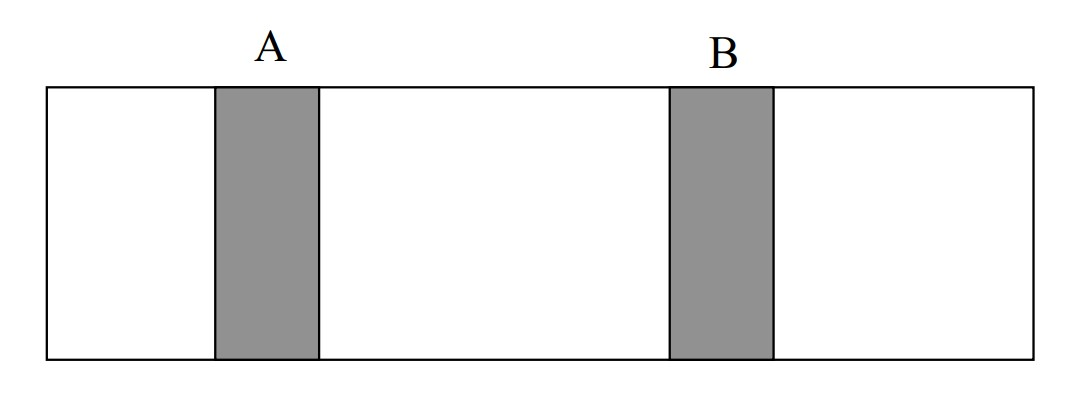
\includegraphics[width=0.5\textwidth]{immagini/AR_proiezione.jpg}
	\caption*{Restrizione $\sigma$\textsubscript{Cond}(R)}
	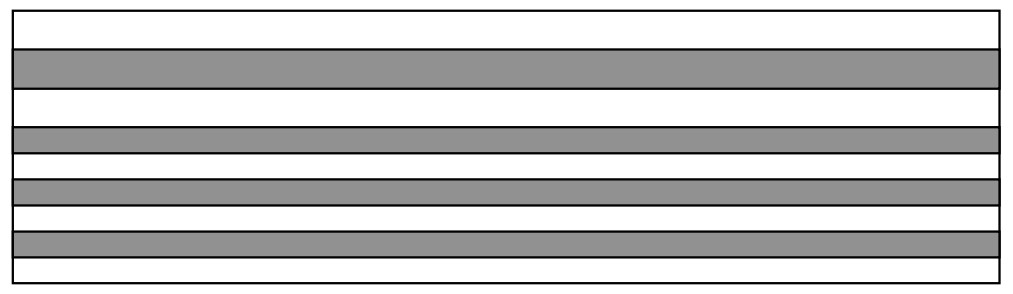
\includegraphics[width=0.5\textwidth]{immagini/AR_selezione.jpg}
\end{figure}

\subsubsection{Prodotto}

Prodotto:\ $R \times S$
\begin{figure}[H]
	\centering
	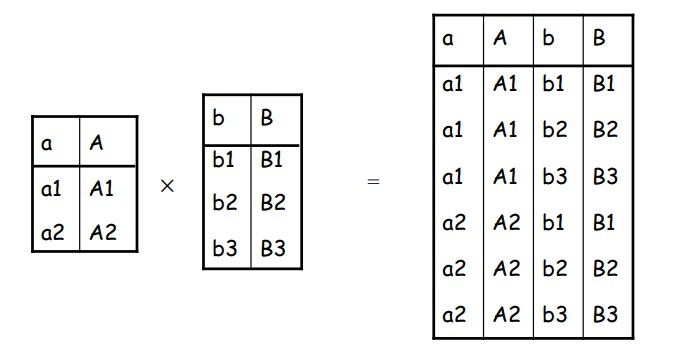
\includegraphics[width=0.5\textwidth]{immagini/AR_prodotto.jpg}
\end{figure}

\subsubsection{Join (giunzione)}

\textit{Combinando selezione e proiezione}, possiamo estrarre informazioni da una relazione, ma \textit{non} possiamo \textit{correlare} informazioni presenti in relazioni diver\-se.\
Il \textbf{join} è l'operatore più interessante dell'algebra relazionale poiché permette di \textbf{correlare} dati in relazioni diverse.

\subsubsection{Join naturale}
Operatore binario (generalizzabile) che correla dati in relazioni diverse, \textbf{sulla base di valori uguali in attributi con lo stesso nome}.\
Produce un risultato:
\begin{itemize}
	\item sull'unione degli attributi degli operandi;
	\item con ennuple che sono ottenute combinando le ennuple degli operandi con valori uguali sugli attributi in comune.
\end{itemize}
$R_1(X_1)$, $R_2(X_2)$

\noindent $R_1 \Join R_2$ è una relazione su $X_1 \cup X_2$.

\[R_1 \Join R_2 =\]
\[     \{ t\ su\ X_1 \cup X_2\ |\ \mathrm{esistono}\ t_1 \in R_1\ \mathrm{e}\ t_2\in R_2\ \mathrm{con}\ t[X_1] = t_1\ \mathrm{e}\ t[X_2] = t_2 \}
\]
Se ogni ennupla contribuisce al risultato:\ join completo.

\subsubsection{Cardinalità del join}

Il join di $R_1$ e $R_2$ contiene un numero di ennuple compreso fra zero e il prodotto
di $|R_1|$ e $|R_2|$:

\[ 0 \leq |R_1 \Join R_2 | \leq | R_1 | \times | R_2 | \]
Se il join fra $R_1$ ed $R_2$ è completo, allora contiene un numero di ennuple almeno uguale al massimo fra $|R_1|$ e $|R_2|$.\
Se il join coinvolge una chiave $B$ di $R_2$, allora il numero di ennuple è compreso fra zero e $|R_1|$:

\[ 0 \leq |R_1 \Join R_2 | \leq | R_1 |\]

\noindent Se il join coinvolge una chiave $B$ di $R_2$ e un vincolo di integrità referenziale tra attributi di $R_1$ ($B \in R_1$) e la chiave di $R_2$, allora il numero di ennuple è pari a $|$R\textsubscript{1}$|$:
\[|R_1 \Join R_2 | = | R_1 | \]

\subsubsection{Join esterno}
Il \textbf{join esterno} estende, con valori nulli, le ennuple che verrebbero tagliate fuori da un join (\textbf{interno}).\
Esiste in tre versioni:\ sinistro, destro, completo.
\begin{itemize}
	\item Sinistro:\ mantiene tutte le ennuple del primo operando, estendendole con valori nulli, se necessario \qquad $R\stackrel{\leftarrow}{\Join}S$
	\item destro:\ \dots del secondo operando\dots \qquad $R\stackrel{\rightarrow}{\Join}S$
	\item completo:\ \dots di entrambi gli operandi \dots \qquad $R\stackrel{\leftrightarrow}{\Join}S$
\end{itemize}

\noindent\textbf{Nota bene}:\
\[\pi_{X_1}(R_1 \Join R_2) \subseteq R_1\]
\[R \supseteq (\pi_{X_1}(R)) \Join (\pi_{X_2}(R))\]

\subsubsection{Prodotto cartesiano}

Un join naturale su relazioni senza attributi in comune.\
Contiene sempre un numero di ennuple pari al prodotto delle cardinalità degli operandi (le ennuple sono tutte combinabili).

Poiché il prodotto cartesiano concatena tuple non necessariamente correlate dal punto di vista semantico, in pratica, ha senso solo se seguito da selezione:
\[\sigma_{\mathrm{Condizione}} (R_1 \Join R_2)\]
L'operazione viene chiamata \textbf{theta-join} e può essere sintatticamente indicata con
\[R_1 \Join_{\mathrm{Condizione}} R_2\]
Le due scritture sono equivalenti.

La condizione C è spesso una congiunzione ($\land$) di atomi di confronto $A_1\ \vartheta\ A_2$, dove $\vartheta$ è uno degli operatori di confronto ($=, > , <, \dots$).\
Se l'operatore è sempre l'uguaglianza ($=$) allora si parla di \textbf{equi-join}.

\subsubsection{Self Join}
Supponiamo di considerare la seguente relazione

\begin{table}[H]
	\centering
	\begin{tabular}{|l|l|}
		\hline
		\textbf{Genitore} & \textbf{Figlio} \\\hline\hline
		Luca              & Anna            \\\hline
		Maria             & Anna            \\\hline
		Giorgio           & Luca            \\\hline
		Silvia            & Maria           \\\hline
		Enzo              & Maria           \\\hline
	\end{tabular}
\end{table}
\noindent e di volere ottenere una relazione Nonno-Nipote.\
È ovvio che in questo caso abbiamo bisogno di utilizzare due volte la stessa tabella.\
Tuttavia Genitore $\Join$ Genitore = Genitore, poiché tutti gli attributi coincidono.
In questo caso è utile effettuare una ridenominazione:
\begin{center}
	$\rho$\textsubscript{Nonno, Genitore $\leftarrow$ Genitore, Figlio}(Genitore)
\end{center}
A questo punto effettuando un \textit{natural join} con la tabella Genitore, si ottiene l'informazione cercata.
\begin{figure}[H]
	\centering
	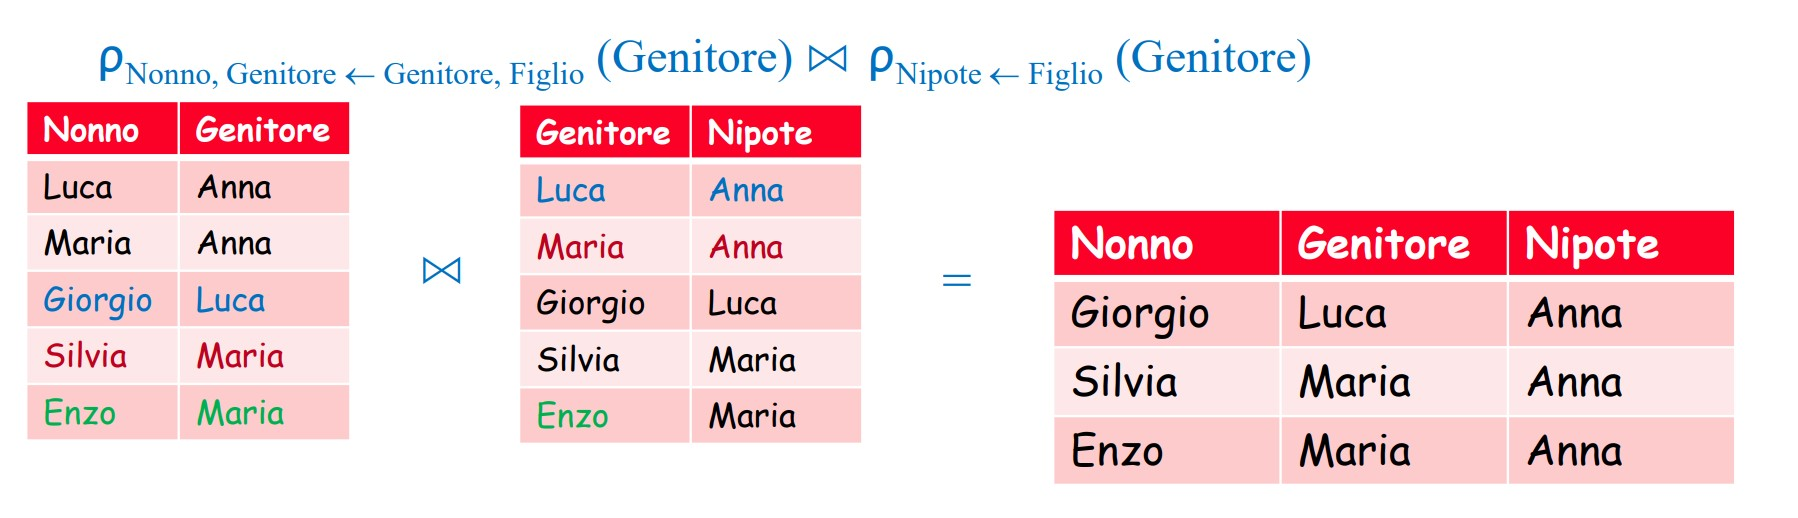
\includegraphics[width=\textwidth]{immagini/AR_SelfJoin.jpg}
\end{figure}
\noindent Eventualmente si può effettuare una proiezione
\begin{figure}[H]
	\centering
	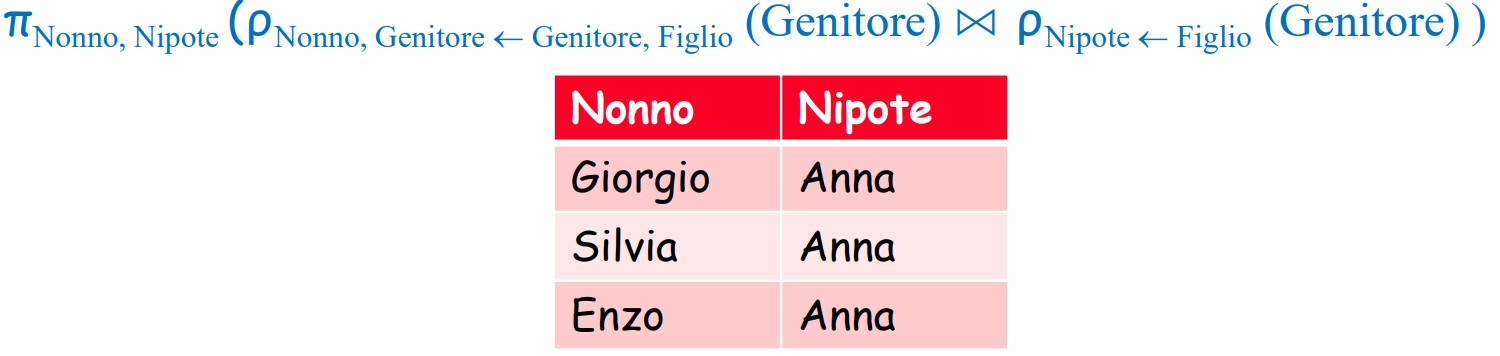
\includegraphics[width=0.9\textwidth]{immagini/AR_SelfJoin2.jpg}
\end{figure}

\subsubsection{Raggruppamento}

Raggruppamento:\ $ _{\{A_i\}}\gamma_{\{f_i\}}(R)$

Gli A\textsubscript{i} sono attributi di $R$ e le $f_i$ sono espressioni che usano funzioni di aggregazione (\texttt{min}, \texttt{max}, \texttt{count}, \texttt{sum},\ \dots).\
Il valore del raggruppamento è una relazione calcolata come segue:
\begin{itemize}
	\item Si partizionano le ennuple di $R$ mettendo nello stesso gruppo tutte le ennuple con valori uguali degli $A_i$.
	\item Si calcolano le espressioni $f_i$ per ogni gruppo.
	\item Per ogni gruppo si restituisce una sola ennupla con attributi i valori degli $A_i$ e delle espressioni $f_i$
\end{itemize}

\begin{figure}[H]
	\centering
	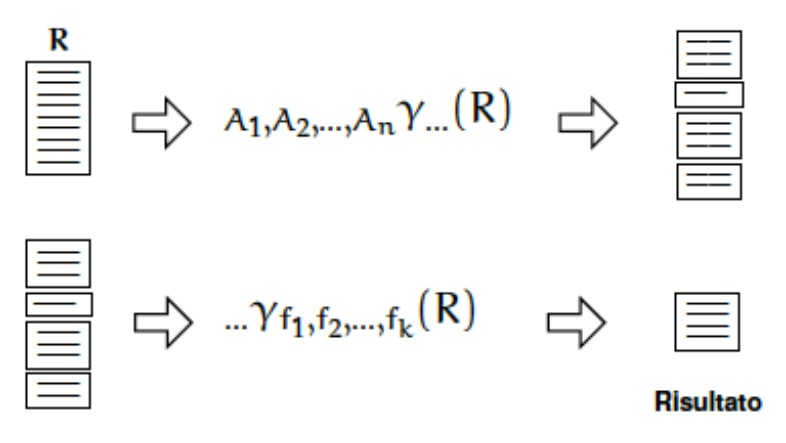
\includegraphics[width=0.5\textwidth]{immagini/Raggruppamento.jpg}
\end{figure}

\subsection{Trasformazioni Algebriche}

Basate su regole di equivalenza fra espressione algebriche, consentono di scegliere diversi ordini di join e di anticipare proiezioni e restrizioni.\
Alcuni esempi con la relazione $R(A, B, C, D)$:

$\pi_A(\pi_{A,B}(R)) \equiv \pi_A(R)$

$\sigma_{C_1}(\sigma_{C_2}(R)) \equiv \sigma_{C_1 \land C_2}(R)$

$\sigma_{C_1 \land C_2}(R \times S) \equiv \sigma_{C_1}(R) \times \sigma_{C_2}(S) $

$R \times (S \times T) \equiv (R \times S) \times T$

$(R \times S) \equiv (S \times R)$

$_X\gamma_F(\sigma_C(R)) \equiv \sigma_C(_X\gamma_F(R) $

\subsubsection{Non distributività della proiezione rispetto alla differenza}

In generale, se $R_1$ e $R_2$ sono definite su $AB$, e contengono tuple uguali su $A$ e diverse su $B$.
\[\pi_A(R_1-R_2) \neq \pi_A(R_1)-\pi_A(R_2)\]


\subsubsection{Operatori algebrici non insiemistici}

$\pi^b_{\{A_i\}}(R)$:\ proiezione multiinsiemistica (senza eliminazione dei duplicati)

\noindent$\tau_{\{Ai\}}(R)$:\ ordinamento

\subsection{Calcolo relazionale su ennuple}

Il calcolo relazionale è un linguaggio che permette di definire il risultato di un'interrogazione come l'insieme di quelle ennuple che soddisfano una certa condizione $\phi$.\
L'insieme delle matricole degli studenti che hanno superato qualcuno degli esami elencati nella relazione Materie(Materia), si può definire come:\
\begin{table}[H]
	\centering
	\begin{tabular}{l c l}
		\{t.matricola & $|$ & t $\in$ Studenti, $\exists$m $\in$ Materie. $\exists$e $\in$ ProveEsami. \\
		              &     & e.Candidato = t.Matricola $\land$ e.Materia = m.Materia\}                \\
	\end{tabular}
\end{table}

\noindent Che è equivalente a

\begin{center}
	$\pi$\textsubscript{Matricola}(Studenti $\Join$\textsubscript{Matricola = Candidato} (ProveEsami $\Join$ Materie))
\end{center}
